% !TEX root = ../main.tex
\chapter{The IS--LM Model}
\label{ch:islm}

The Keynesian cross of Chapter~\ref{ch:keynes} determines output for a \emph{given} interest rate: it tells us where planned expenditure crosses the $45^\circ$ line, but it takes the interest rate $r$ as a number handed down from outside. Yet $r$ is itself an equilibrium price --- the price of liquidity --- and it moves when output moves. The IS--LM model closes this loop. It holds the price level fixed (we are still in the short run) and asks for the pair $(Y,r)$ at which two markets clear simultaneously: the market for goods, summarized by the \emph{IS} curve, and the market for money, summarized by the \emph{LM} curve. Fiscal policy will turn out to act on the first curve and monetary policy on the second, and the interaction of the two is what makes the simple multiplier of the previous chapter an overstatement.

\section{The IS Curve}

The IS curve is the set of all $(Y,r)$ pairs at which the goods market is in equilibrium --- that is, at which planned expenditure equals output. Every point on it is a Keynesian-cross equilibrium for a particular interest rate. To see its shape, recall that investment falls when the interest rate rises, $I=I(r)$ with $I'(r)<0$. Solving the Keynesian cross with investment written as a function of $r$,
\[
Y^{*} = \frac{1}{1-\mathrm{MPC}}\,\big(C_0 - \mathrm{MPC}\cdot T + I(r) + G + \mathrm{NX}\big),
\]
so a lower interest rate raises investment, shifts the planned-expenditure line upward, and --- magnified by the multiplier --- raises equilibrium output. Output and the interest rate therefore move in opposite directions along the goods-market equilibrium locus.

\begin{figure}[h]
\centering
\begin{tikzpicture}[scale=1.0]
  % ---- shared geometry: the two output levels live on one vertical grid ----
  \def\Yzero{2.8}   % Y0
  \def\Yone{5.6}    % Y1
  \def\xmax{7.4}

  % ================= TOP PANEL: Keynesian cross =================
  \begin{scope}[shift={(0,6.6)}]
    % axes
    \draw[-Latex] (0,0) -- (\xmax,0) node[right] {$Y$};
    \draw[-Latex] (0,0) -- (0,6.0) node[above] {$\mathrm{AD}$};
    % 45-degree line (reaches above the upper equilibrium Y1)
    \draw (0,0) -- (5.95,5.95);
    \node[above left=-2pt and -2pt] at (5.95,5.95) {$45^{\circ}$};
    % lower AE line (slope = MPC < 1): crosses 45-line at Y0
    \draw[line width=1.0pt] (0,1.4) -- (6.7,{1.4+0.5*6.7});
    % upper AE line: shifted up, crosses 45-line at Y1
    \draw[line width=1.0pt] (0,2.8) -- (6.0,{2.8+0.5*6.0});
    % equilibrium dots
    \fill (\Yzero,\Yzero) circle (1.5pt);
    \fill (\Yone,\Yone) circle (1.5pt);
    % upward-shift arrow
    \draw[-Latex] (0.85,1.9) to[bend left=32] (1.05,3.05);
    % vertical guides down to the Y axis
    \draw[densely dashed] (\Yzero,\Yzero) -- (\Yzero,0) node[below] {$Y_{0}$};
    \draw[densely dashed] (\Yone,\Yone)   -- (\Yone,0)   node[below] {$Y_{1}$};
  \end{scope}

  % ================= BOTTOM PANEL: the IS curve =================
  \begin{scope}[shift={(0,0)}]
    % axes
    \draw[-Latex] (0,0) -- (\xmax,0) node[right] {$Y$};
    \draw[-Latex] (0,0) -- (0,4.8) node[above] {$r$};
    % downward-sloping convex IS curve
    \def\rzero{3.0}  % r0 height (above Y0)
    \def\rone{1.3}   % r1 height (above Y1)
    \draw[line width=1.0pt,smooth,samples=120,domain=0.9:7.0]
      plot (\x,{4.6*exp(-0.42*\x)+0.45}) node[right] {$\mathrm{IS}$};
    % equilibrium points on the curve
    \fill (\Yzero,{4.6*exp(-0.42*\Yzero)+0.45}) circle (1.5pt);
    \fill (\Yone,{4.6*exp(-0.42*\Yone)+0.45}) circle (1.5pt);
    % vertical guides up to the top panel and down to the Y axis
    \draw[densely dashed] (\Yzero,4.8) -- (\Yzero,0) node[below] {$Y_{0}$};
    \draw[densely dashed] (\Yone,4.8)  -- (\Yone,0)  node[below] {$Y_{1}$};
    % horizontal guides marking r0 and r1
    \draw[densely dashed] (0,{4.6*exp(-0.42*\Yzero)+0.45}) -- (\Yzero,{4.6*exp(-0.42*\Yzero)+0.45});
    \draw[densely dashed] (0,{4.6*exp(-0.42*\Yone)+0.45})  -- (\Yone,{4.6*exp(-0.42*\Yone)+0.45});
    \node[left] at (0,{4.6*exp(-0.42*\Yzero)+0.45}) {$r_{0}$};
    \node[left] at (0,{4.6*exp(-0.42*\Yone)+0.45})  {$r_{1}$};
    % downward arrow on the r axis from r0 to r1
    \draw[-Latex] (-0.95,{4.6*exp(-0.42*\Yzero)+0.45}) to[bend right=30] (-0.95,{4.6*exp(-0.42*\Yone)+0.45+0.05});
  \end{scope}
\end{tikzpicture}

\caption{Deriving the IS curve. In the upper panel a fall in the interest rate from $r_0$ to $r_1$ raises investment, shifting planned expenditure up and moving the Keynesian-cross equilibrium from $Y_0$ to $Y_1$. Plotting each interest rate against the output it implies (lower panel) traces out the downward-sloping IS curve.}
\label{fig:macro-15}
\end{figure}

\defn{The IS Curve}{
The \emph{IS curve} is the locus of $(Y,r)$ pairs at which planned expenditure equals output (the goods market clears). Because a lower interest rate raises investment and hence equilibrium output, the IS curve slopes \emph{downward}.
}

Figure~\ref{fig:macro-15} stacks the two panels that produce it. Anything other than the interest rate that shifts the Keynesian-cross equilibrium --- a change in $G$, in taxes, in autonomous consumption or investment, or in net exports --- shifts the \emph{whole} IS curve; a change in the interest rate is a movement \emph{along} it.

\section{The LM Curve}

The LM curve comes from the money market. The quantity theory, $MV = PY$, can be read as a statement about money demand: to carry out a nominal volume of transactions $PY$ at a velocity $V$, the public wishes to hold
\[
M^{d} = \frac{PY}{V}.
\]
Velocity is not a constant here; it rises with the interest rate, $V=V(r)$, $V'(r)>0$, because a higher interest rate raises the opportunity cost of holding non-interest-bearing money, so each unit of money is turned over faster and less of it is demanded. The supply of money, by contrast, is set by the central bank and is independent of the interest rate: in the diagram it is a vertical line.

\begin{figure}[h]
\centering
\begin{tikzpicture}[scale=1.0]
  % axes
  \draw[-Latex] (0,0) -- (7.6,0) node[right] {$M$};
  \draw[-Latex] (0,0) -- (0,5.8) node[above] {$r$};
  % vertical money-supply line M^s (perfectly inelastic), thick = primary
  \draw[line width=1.2pt] (4.3,0) -- (4.3,5.4) node[above] {$M^{s}$};
  % downward-sloping money-demand curve M^d : r = k/(M - a)
  % chosen so it crosses M^s at a sensible interior r
  \draw[semithick,domain=0.95:7.2,smooth,variable=\x,samples=160]
        plot ({\x},{1.55/(\x-0.55)+0.18}) node[right] {$M^{d}$};
  % equilibrium point: x=4.3 on the demand curve
  \pgfmathsetmacro{\req}{1.55/(4.3-0.55)+0.18}
  \fill (4.3,\req) circle (1.6pt);
  % dashed guide to the r axis
  \draw[densely dashed] (4.3,\req) -- (0,\req) node[left] {$r^{*}$};
\end{tikzpicture}

\caption{The money market. The money supply $M^{s}$ is vertical (set by the central bank); money demand $M^{d}$ slopes down in the interest rate. Their intersection fixes the equilibrium interest rate.}
\label{fig:macro-16}
\end{figure}

Equilibrium in Figure~\ref{fig:macro-16} pins down the interest rate that clears the money market for a given level of output and prices. Now raise output. Higher $Y$ means more transactions and thus greater money demand at every interest rate, shifting the demand curve to the right. With supply fixed, the interest rate must rise to choke money demand back to the available stock.

\begin{figure}[h]
\centering
\begin{tikzpicture}[scale=1.0]
  % axes
  \draw[-Latex] (0,0) -- (8.6,0) node[right] {$M$};
  \draw[-Latex] (0,0) -- (0,6.4) node[above] {$r$};
  % vertical money supply M^s fixed
  \def\Ms{4.6}
  \draw[line width=1.2pt] (\Ms,0) -- (\Ms,6.0);
  \node[above] at (\Ms,6.0) {$M^{s}$};
  % money demand curves: rectangular-hyperbola shape r = k/M
  % M^{d_1} : original demand, equilibrium r_1 at M = Ms
  \def\rone{1.7}
  \pgfmathsetmacro{\kone}{\rone*\Ms}      % so that k/Ms = r_1
  \draw[semithick,domain=1.55:8.1,smooth,variable=\x,samples=160]
        plot ({\x},{\kone/\x});
  \node[below right] at (8.1,{\kone/8.1}) {$M^{d_1}$};
  % M^{d_2} : higher demand after GDP rises (shifted right), equilibrium r_2 at M = Ms
  \def\rtwo{3.0}
  \pgfmathsetmacro{\ktwo}{\rtwo*\Ms}      % so that k/Ms = r_2
  \draw[semithick,domain=2.35:8.3,smooth,variable=\x,samples=160]
        plot ({\x},{\ktwo/\x});
  \node[right] at (8.3,{\ktwo/8.3}) {$M^{d_2}$};
  % equilibrium points
  \fill (\Ms,\rone) circle (1.6pt);
  \fill (\Ms,\rtwo) circle (1.6pt);
  % dashed guides to the r-axis
  \draw[densely dashed] (\Ms,\rone) -- (0,\rone) node[left] {$r_1$};
  \draw[densely dashed] (\Ms,\rtwo) -- (0,\rtwo) node[left] {$r_2$};
  % upward arrow on the r-axis showing r rises
  \draw[-Latex] (-0.62,\rone) -- (-0.62,\rtwo);
  % single arrow showing the rightward shift of demand (in blank space)
  \draw[-Latex] (5.0,1.55) -- (5.95,2.2);
\end{tikzpicture}

\caption{A rise in output shifts money demand to the right; with the money supply fixed, the equilibrium interest rate rises from $r_0$ to $r_1$.}
\label{fig:macro-17}
\end{figure}

Collecting these $(Y,r)$ pairs --- higher output requiring a higher interest rate to keep the money market in balance --- traces out the LM curve.

\begin{figure}[h]
\centering
\begin{tikzpicture}[scale=1.0]
  % axes
  \draw[-Latex] (0,0) -- (0,5.4) node[above] {$r$};
  \draw[-Latex] (0,0) -- (7.6,0) node[right] {$Y$};
  % LM curve: upward-sloping convex locus, nearly flat at low Y, steep at high Y
  \draw[line width=1.2pt,smooth,samples=120,domain=0.5:6.2]
        plot (\x,{0.7+0.085*(\x-0.5)^2});
  \node[right] at (6.25,{0.7+0.085*(6.2-0.5)^2}) {$\mathrm{LM}$};
\end{tikzpicture}

\caption{The LM curve: the locus of output and interest-rate pairs at which the money market clears. It slopes upward because higher output raises money demand and hence the market-clearing interest rate.}
\label{fig:macro-18}
\end{figure}

\defn{The LM Curve}{
The \emph{LM curve} (liquidity preference--money supply) is the locus of $(Y,r)$ pairs at which the money market clears for a given real money supply. Because higher output raises money demand and therefore the equilibrium interest rate, the LM curve slopes \emph{upward}.
}

What shifts the entire LM curve? Anything that changes the real money supply $M/P$. An increase in the nominal money supply means that, at any level of output, the market clears at a lower interest rate, so the LM curve shifts down (equivalently, to the right).

\begin{figure}[h]
\centering
\begin{tikzpicture}[scale=1.0]
  %================ LEFT PANEL: money market ================
  \begin{scope}[shift={(0,0)}]
    % axes
    \draw[-Latex] (0,0) -- (6.4,0) node[right] {$M$};
    \draw[-Latex] (0,0) -- (0,5.6) node[above] {$r$};
    % money demand M^d : downward-sloping convex curve (rectangular hyperbola)
    \draw[semithick,smooth,samples=120,domain=0.62:5.9,variable=\x]
          plot ({\x},{2.7/(\x-0.25)+0.55}) ;
    \node[right] at (5.55,0.95) {$M^{d}$};
    % two vertical money-supply lines
    \def\Msa{3.3}\def\Msb{4.6}
    \draw[semithick] (\Msa,0) -- (\Msa,5.1) node[above] {$M^{s_{1}}$};
    \draw[semithick] (\Msb,0) -- (\Msb,5.1) node[above] {$M^{s_{2}}$};
    % equilibrium interest rates: r1 at inner supply, r2 (lower) at outer supply
    \pgfmathsetmacro{\rone}{2.7/(\Msa-0.25)+0.55}
    \pgfmathsetmacro{\rtwo}{2.7/(\Msb-0.25)+0.55}
    \fill (\Msa,\rone) circle (1.5pt);
    \fill (\Msb,\rtwo) circle (1.5pt);
    \draw[densely dashed] (0,\rone) -- (\Msa,\rone);
    \draw[densely dashed] (0,\rtwo) -- (\Msb,\rtwo);
    \node[left] at (0,\rone) {$r_{1}$};
    \node[left] at (0,\rtwo) {$r_{2}$};
  \end{scope}

  %================ connector ================
  \node at (7.6,2.7) {\Large $\Rightarrow$};

  %================ RIGHT PANEL: LM shift ================
  \begin{scope}[shift={(8.8,0)}]
    % axes
    \draw[-Latex] (0,0) -- (6.4,0) node[right] {$Y$};
    \draw[-Latex] (0,0) -- (0,5.6) node[above] {$r$};
    % upper (original) LM curve
    \draw[semithick,smooth,samples=120,domain=0.7:4.2,variable=\x]
          plot ({\x},{0.30*(\x-0.4)*(\x-0.4)+0.9});
    % lower/right (shifted) LM curve
    \draw[semithick,smooth,samples=120,domain=1.7:5.3,variable=\x]
          plot ({\x},{0.30*(\x-1.4)*(\x-1.4)+0.55});
    \node[above right] at (4.05,4.85) {$\mathrm{LM}$};
    % small shift arrows sitting in the blank gap between the two LM curves,
    % pointing down/right (direction of the shift) without touching either curve
    \draw[-Latex,semithick] (2.6,2.05) -- (2.95,1.6);
    \draw[-Latex,semithick] (3.4,3.0) -- (3.75,2.55);
  \end{scope}
\end{tikzpicture}

\caption{An increase in the money supply (from $M^{s_1}$ to $M^{s_2}$) lowers the market-clearing interest rate at each level of output, shifting the LM curve down and to the right.}
\label{fig:macro-19}
\end{figure}

A rise in the price level works in the opposite direction. The relevant quantity is the \emph{real} money supply $M/P$: a higher $P$ shrinks $M/P$ exactly as a cut in the nominal money supply would, raising money demand relative to supply and pushing the LM curve up.

\begin{figure}[h]
\centering
\begin{tikzpicture}[scale=1.0]
  % ============================ LEFT PANEL: money market ============================
  \begin{scope}
    % axes
    \draw[-Latex] (0,0) -- (6.2,0) node[right] {$M$};
    \draw[-Latex] (0,0) -- (0,5.6) node[above] {$r$};
    % vertical money supply M^s
    \draw[line width=1.0pt] (3.9,0) -- (3.9,5.3);
    \node[above] at (3.9,5.3) {$M^{s}$};
    % money demand M^{d1} (lower/left convex curve): hyperbola passing through (3.9, r1)
    % r1 = 1.5 at M=3.9  => k1 = 1.5*3.9 = 5.85
    \draw[smooth,samples=120,domain=1.18:5.9,variable=\x] plot ({\x},{5.85/\x});
    \node[below right] at (5.9,5.85/5.9) {$M^{d1}$};
    % money demand M^{d2} (upper/right convex curve): hyperbola passing through (3.9, r2)
    % r2 = 2.85 at M=3.9  => k2 = 2.85*3.9 = 11.115
    \draw[smooth,samples=120,domain=2.05:5.9,variable=\x] plot ({\x},{11.115/\x});
    \node[below right] at (5.9,11.115/5.9) {$M^{d2}$};
    % equilibrium points on the M^s line
    \fill (3.9,1.5) circle (1.4pt);
    \fill (3.9,2.85) circle (1.4pt);
    % dashed horizontal guides to the r-axis
    \draw[densely dashed] (0,1.5) -- (3.9,1.5);
    \draw[densely dashed] (0,2.85) -- (3.9,2.85);
    \node[left] at (0,1.5) {$r_1$};
    \node[left] at (0,2.85) {$r_2$};
    % up-arrow on the r-axis between r1 and r2
    \draw[-Latex] (0.42,1.55) -- (0.42,2.80);
    % small arrows in the blank gap between M^{d1} and M^{d2}, indicating the rightward/upward shift
    \draw[-Latex] (2.0,3.55) -- (2.5,4.05);
    \draw[-Latex] (2.85,2.6) -- (3.35,2.95);
  \end{scope}

  % ============================ CONNECTOR ============================
  \node[scale=2.4] at (7.5,2.6) {$\Rightarrow$};

  % ============================ RIGHT PANEL: LM curve ============================
  \begin{scope}[xshift=9.0cm]
    % axes
    \draw[-Latex] (0,0) -- (6.2,0) node[right] {$Y$};
    \draw[-Latex] (0,0) -- (0,5.6) node[above] {$r$};
    % lower LM curve (convex, upward sloping): r = 0.55 + 0.10*(Y)^2 over a shifted range
    \draw[smooth,samples=120,domain=0.4:5.2,variable=\x]
        plot ({\x},{0.55+0.135*(\x)*(\x)});
    % upper LM curve: same shape shifted up by ~0.9
    \draw[smooth,samples=120,domain=0.4:4.85,variable=\x]
        plot ({\x},{1.45+0.135*(\x)*(\x)});
    \node[above left] at (4.85,1.45+0.135*4.85*4.85) {$\mathrm{LM}$};
    % small up-arrows in the blank gap between the two LM curves (clear of both)
    \draw[-Latex] (2.55,0.55+0.135*2.55*2.55+0.20) -- (2.55,1.45+0.135*2.55*2.55-0.14);
    \draw[-Latex] (3.65,0.55+0.135*3.65*3.65+0.20) -- (3.65,1.45+0.135*3.65*3.65-0.14);
  \end{scope}
\end{tikzpicture}

\caption{A rise in the price level raises nominal money demand (lowers the real money supply $M/P$); the market-clearing interest rate rises at each level of output and the LM curve shifts up.}
\label{fig:macro-20}
\end{figure}

\state{Reading the two curves}{
The IS curve summarizes the goods market and is shifted by \emph{fiscal} variables ($G$, $T$, autonomous spending). The LM curve summarizes the money market and is shifted by \emph{monetary} variables --- the nominal money supply and the price level, both acting through the real money supply $M/P$.
}

\section{Equilibrium}

Plotting the two curves together, with output on the horizontal axis and the interest rate on the vertical axis, the unique crossing point gives the pair $(Y_0,r_0)$ at which \emph{both} markets clear. The arrow of causation runs both ways: the interest rate helps determine output through investment, and output helps determine the interest rate through money demand.

\begin{figure}[h]
\centering
\begin{tikzpicture}[scale=1.0]
  % axes
  \draw[-Latex] (0,0) -- (8.2,0) node[right] {$Y$};
  \draw[-Latex] (0,0) -- (0,6.0) node[above] {$r$};
  % IS curve: downward sloping
  \draw[line width=1pt] (1.1,4.7) -- (6.6,1.0) node[below right] {$\mathrm{IS}$};
  % LM curve: upward sloping
  \draw[line width=1pt] (1.1,1.4) -- (7.0,5.1) node[above right] {$\mathrm{LM}$};
  % equilibrium intersection: solve the two lines
  % IS: from (1.1,4.7) to (6.6,1.0): slope = (1.0-4.7)/(6.6-1.1) = -0.6727, r = 4.7 -0.6727(Y-1.1)
  % LM: from (1.1,1.4) to (7.0,5.1): slope = (5.1-1.4)/(7.0-1.1) = 0.6271, r = 1.4 +0.6271(Y-1.1)
  % set equal: 4.7 -0.6727(Y-1.1) = 1.4 +0.6271(Y-1.1)
  % 3.3 = 1.2998(Y-1.1) -> Y-1.1 = 2.539 -> Y = 3.639, r = 1.4+0.6271*2.539 = 2.992
  \coordinate (E) at (3.639,2.992);
  \fill (E) circle (1.7pt);
  % dashed guide down to Y axis
  \draw[densely dashed] (E) -- (3.639,0) node[below] {$Y_0$};
  % dashed guide to r axis
  \draw[densely dashed] (E) -- (0,2.992) node[left] {$r_0$};
\end{tikzpicture}

\caption{IS--LM equilibrium: the downward-sloping IS curve and the upward-sloping LM curve cross at the unique pair $(Y_0,r_0)$ at which both the goods and money markets clear.}
\label{fig:macro-21}
\end{figure}

The equilibrium is stable. Suppose some force pushed output above $Y_0$ --- say a policy interest rate set too low. At that higher output, money demand would outstrip the fixed supply and the interest rate would be bid up, choking off investment until output returned to the equilibrium. A change in the interest rate or in output moves the economy \emph{along} the curves; a change in any other determinant shifts a curve bodily.

\section{Fiscal Policy in IS--LM}

Consider an increase in government purchases. In the goods market this shifts the IS curve to the right. If the interest rate stayed at $r_0$, output would rise all the way to $Y_1$, the full Keynesian-cross multiplier acting on the larger $G$. But the move along the new IS curve toward its intersection with the unchanged LM curve tells a more sober story: as output rises, money demand rises, the interest rate is pushed up to $r_2$, and the higher interest rate crowds out private investment, pulling output back from $Y_1$ to $Y_2$, with $Y_0<Y_2<Y_1$.

\begin{figure}[h]
\centering
\input{figures/fig22}
\caption{A rise in government purchases shifts the IS curve to the right. At a fixed interest rate output would reach $Y_1$; but the induced rise in the interest rate to $r_2$ crowds out investment, so the new equilibrium is at $Y_2$, with $Y_0<Y_2<Y_1$. The gap $Y_1-Y_2$ is the first crowding-out effect.}
\label{fig:macro-22}
\end{figure}

\defn{The (First) Crowding-Out Effect}{
The \emph{crowding-out effect} is the reduction in private investment caused by the rise in the interest rate that a fiscal expansion induces through the money market. It makes the realized output gain ($Y_2-Y_0$) smaller than the naive multiplier prediction ($Y_1-Y_0$).
}

A tax cut shifts the IS curve outward in the same way (through the tax multiplier rather than the spending multiplier), and the same crowding-out logic applies. The unifying statement is that \emph{fiscal policy acts on the IS curve}.

\section{Monetary Policy in IS--LM}

Now let the central bank increase the money supply. The IS curve is unaffected; the LM curve shifts down, because more money clears the market at a lower interest rate for any output. At the initial output the interest rate would fall; the lower rate stimulates investment and output rises along the IS curve to $Y_1$, with a new, lower equilibrium interest rate $r_1$.

\begin{figure}[h]
\centering
% original hand-drawn figure (kept as-is per author; TikZ parked in fig23_tikz.txt)
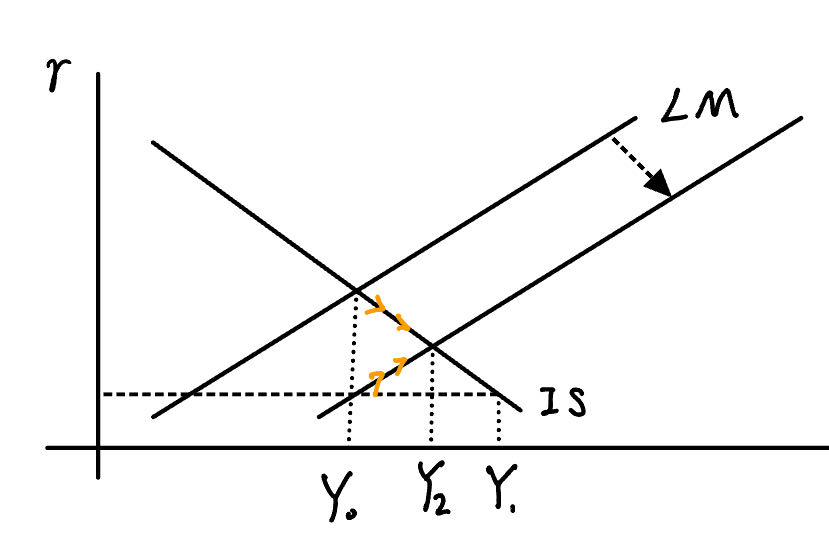
\includegraphics[width=\linewidth,height=0.9\textheight,keepaspectratio]{figures/fig23.png}

\caption{An increase in the money supply shifts the LM curve down. Output rises from $Y_0$ to $Y_1$ and the interest rate falls from $r_0$ to $r_1$.}
\label{fig:macro-23}
\end{figure}

A rise in the price level runs the same machinery in reverse. Because it reduces the real money supply $M/P$, it shifts the LM curve up, raising the interest rate and lowering output.

\begin{figure}[h]
\centering
% original hand-drawn figure (kept as-is per author; TikZ parked in fig24_tikz.txt)
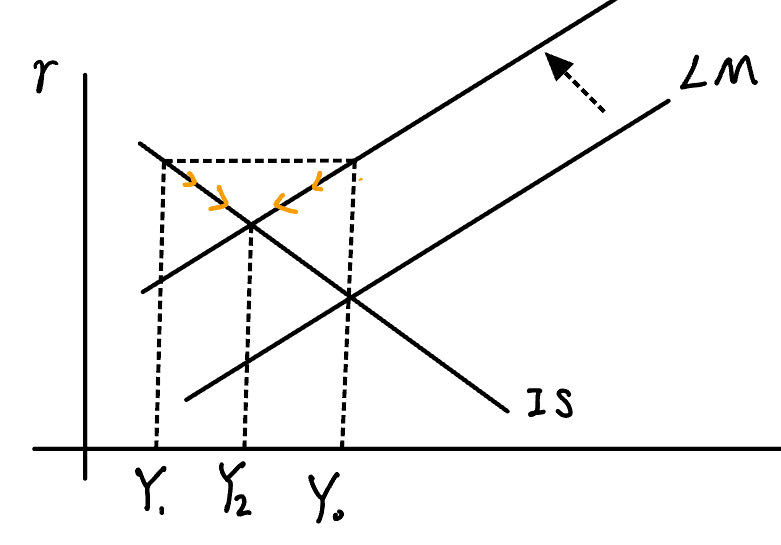
\includegraphics[width=\linewidth,height=0.9\textheight,keepaspectratio]{figures/fig24.png}

\caption{A rise in the price level (a fall in the real money supply $M/P$) shifts the LM curve up: the interest rate rises to $r_1$ and output falls to $Y_1$.}
\label{fig:macro-24}
\end{figure}

This last experiment is worth pausing on, because it is the hinge between IS--LM and the aggregate-demand curve of the next chapter: \emph{a higher price level is equivalent, for the money market, to a smaller money supply}. Holding the nominal money stock fixed and varying $P$ therefore traces a relationship between the price level and equilibrium output --- which is exactly aggregate demand.

\state{Summary}{
Fiscal policy shifts the IS curve; monetary policy (and the price level) shift the LM curve. A fiscal expansion raises output but also the interest rate, crowding out investment; a monetary expansion raises output by lowering the interest rate. In every case the interest rate adjusts so that both markets clear at once.
}
